%% Supplementary Material (v3). Generated tables: make_assets.py
\documentclass[11pt]{article}
\usepackage[a4paper,margin=2.2cm]{geometry}
\usepackage[T1]{fontenc}
\usepackage{lmodern,amsmath,amssymb,booktabs,graphicx,xcolor,microtype,xspace}
\usepackage[hidelinks]{hyperref}
\usepackage{caption}
\captionsetup{font=small,labelfont=bf}
\renewcommand{\thetable}{S\arabic{table}}
\renewcommand{\thefigure}{S\arabic{figure}}
% Generated by make_assets.py - do not edit
\newcommand{\absPenQuic}{106}
\newcommand{\absPenTcp}{105}
\newcommand{\appDeltaErr}{4.1}
\newcommand{\appDpopEC}{518}
\newcommand{\appDpopML}{8{,}206}
\newcommand{\appXmlErr}{0.7}
\newcommand{\baseSixHi}{141}
\newcommand{\baseSixLo}{397}
\newcommand{\baseSwiftMs}{121.5}
\newcommand{\beML}{0.08}
\newcommand{\beMLmbs}{13}
\newcommand{\beRSA}{1.70}
\newcommand{\beSLHf}{0.02}
\newcommand{\blerSixHi}{9}
\newcommand{\blerSixLo}{12}
\newcommand{\busyWarmBase}{31}
\newcommand{\busyWarmML}{34}
\newcommand{\capEC}{15{,}129}
\newcommand{\capHyb}{11{,}614}
\newcommand{\capHybPct}{30}
\newcommand{\capML}{2{,}845}
\newcommand{\capMLm}{2{,}012}
\newcommand{\capMLratio}{5.3}
\newcommand{\ccMatHi}{21}
\newcommand{\ccMatLo}{5}
\newcommand{\ccMaxRttML}{1.00}
\newcommand{\ccRedEC}{31}
\newcommand{\ccRedFal}{12}
\newcommand{\ccRedML}{5}
\newcommand{\ccRedRSA}{22}
\newcommand{\ccRedSLHf}{2}
\newcommand{\certErrMax}{0.8}
\newcommand{\ciMLHi}{3.86}
\newcommand{\ciMLLo}{3.85}
\newcommand{\ciMaxHalf}{15.7}
\newcommand{\compErrPQ}{5}
\newcommand{\compRealECfour}{0.40}
\newcommand{\compRealPQhi}{0.98}
\newcommand{\compRealPQlo}{0.88}
\newcommand{\compositeDepthDelta}{60.4}
\newcommand{\compositeDepthDeltaIdeal}{32.8}
\newcommand{\compositeExtraPct}{0.3}
\newcommand{\desFlows}{126{,}360}
\newcommand{\desMaxDiff}{1.3\times10^{-11}}
\newcommand{\dlFrHi}{2.3}
\newcommand{\dlSixHi}{411}
\newcommand{\dlSixLo}{2.5}
\newcommand{\dlThzHi}{4.3}
\newcommand{\dlUrHi}{42}
\newcommand{\ecCpuMs}{0.5}
\newcommand{\ecDepthDelta}{29.6}
\newcommand{\ecDepthDeltaIdeal}{0.6}
\newcommand{\effSlowdown}{2.0}
\newcommand{\falDepthDelta}{1.2}
\newcommand{\falDepthPen}{0}
\newcommand{\falSignMeas}{0.10}
\newcommand{\falSwiftMs}{123.1}
\newcommand{\fullSfML}{16{,}841}
\newcommand{\harmEmbEC}{0}
\newcommand{\harmEmbML}{95}
\newcommand{\harmEmbRSA}{31}
\newcommand{\harmEmbSLHf}{100}
\newcommand{\harmSrvEC}{0}
\newcommand{\harmSrvML}{0}
\newcommand{\harmSrvRSA}{0}
\newcommand{\harmSrvSLHf}{0}
\newcommand{\hsResidHi}{1.1}
\newcommand{\hsResidLo}{-0.1}
\newcommand{\hybDepthDelta}{29.6}
\newcommand{\hybKneeBase}{121}
\newcommand{\hybKneeBaseIdeal}{121}
\newcommand{\hybKneeHyb}{122}
\newcommand{\hybKneeHybIdeal}{92}
\newcommand{\hybridDeltaKB}{2.2}
\newcommand{\hybridDeltaMs}{0.2}
\newcommand{\icwTenECdOne}{92.1}
\newcommand{\icwTenMLdOne}{127.3}
\newcommand{\icwThirtyTwoECdOne}{92.1}
\newcommand{\icwThirtyTwoMLDelta}{29.9}
\newcommand{\icwThirtyTwoMLdOne}{98.2}
\newcommand{\idleWarmML}{92}
\newcommand{\inetCf}{2.9}
\newcommand{\inetCfHi}{4.4}
\newcommand{\inetCfLo}{1.2}
\newcommand{\inetCfRtt}{30}
\newcommand{\inetGg}{2.5}
\newcommand{\inetGgHi}{5.7}
\newcommand{\inetGgLo}{0.1}
\newcommand{\inetGgRtt}{34}
\newcommand{\inetN}{400}
\newcommand{\lossFactorTwo}{1.71}
\newcommand{\lossFactorZero}{1.69}
\newcommand{\lossGapTwo}{144}
\newcommand{\lossGapZero}{105}
\newcommand{\lossSlhGapTwo}{474}
\newcommand{\lossThzLo}{0.81}
\newcommand{\meanMmBase}{169}
\newcommand{\metaLargeECDelta}{1}
\newcommand{\mitCiRadioHi}{1.29}
\newcommand{\mitCiRadioLo}{3.75}
\newcommand{\mitCiShare}{66}
\newcommand{\mitCiWired}{1.45}
\newcommand{\mitMtcRadioHi}{1.29}
\newcommand{\mitMtcRadioLo}{3.76}
\newcommand{\mitMtcShare}{54}
\newcommand{\mitMtcWired}{1.49}
\newcommand{\mitNoneRadioHi}{1.49}
\newcommand{\mitNoneRadioLo}{3.85}
\newcommand{\mitNoneWired}{1.69}
\newcommand{\mitQuicResWired}{1.13}
\newcommand{\mitQuicSaveMs}{30}
\newcommand{\mitQuicWired}{1.50}
\newcommand{\mitResRadioHi}{1.11}
\newcommand{\mitResRadioLo}{3.18}
\newcommand{\mitResWired}{1.33}
\newcommand{\mlCpuMs}{3.4}
\newcommand{\mlDepthCpu}{0.6}
\newcommand{\mlDepthDelta}{60.0}
\newcommand{\mlDepthDeltaEightSeven}{32.3}
\newcommand{\mlDepthDeltaEightSevenIdeal}{32.1}
\newcommand{\mlDepthDeltaIdeal}{59.9}
\newcommand{\mlDepthNet}{30.5}
\newcommand{\mlDepthSer}{2.9}
\newcommand{\mlDepthSsw}{56.5}
\newcommand{\mlSixHi}{210}
\newcommand{\mlSixLo}{1531}
\newcommand{\mlSswFirstDepth}{1}
\newcommand{\mlSwiftMs}{186.1}
\newcommand{\mldsaSignOqs}{0.27}
\newcommand{\mldsaSignOssl}{0.59}
\newcommand{\mldsaSignVone}{0.22}
\newcommand{\nCold}{140{,}400}
\newcommand{\nConfigs}{175{,}500}
\newcommand{\nRadioRows}{5{,}460}
\newcommand{\nRadioTx}{5{,}460{,}000}
\newcommand{\nTrials}{1{,}000}
\newcommand{\nocertMLKB}{67.2}
\newcommand{\nocertWarmML}{33}
\newcommand{\pNineNineMmBase}{1026}
\newcommand{\perCertNet}{10.2}
\newcommand{\perCertNineZeroZeroZeropTwoFour}{9.1}
\newcommand{\perCertNineZeroZeroZeropZero}{1.1}
\newcommand{\perCertOneFiveZeroZeropTwoFour}{20.0}
\newcommand{\perCertOneFiveZeroZeropZero}{20.0}
\newcommand{\perCertOneTwoEightZeropTwoFour}{10.5}
\newcommand{\perCertOneTwoEightZeropZero}{10.5}
\newcommand{\perCertRttFive}{3.3}
\newcommand{\perCertRttOneZeroZero}{66.7}
\newcommand{\quicGateTen}{0.5}
\newcommand{\quicGateThirtyTwo}{30}
\newcommand{\radDepthFourHi}{1.52}
\newcommand{\radDepthFourZero}{3.47}
\newcommand{\radDepthOneHi}{1.12}
\newcommand{\radDepthOneZero}{2.86}
\newcommand{\ratioECHundred}{57.1}
\newcommand{\ratioMLhundred}{27}
\newcommand{\ratioSLHsHundred}{0.1}
\newcommand{\resChML}{7{,}849}
\newcommand{\resSfML}{1{,}297}
\newcommand{\resTicketBase}{208}
\newcommand{\resTicketML}{6{,}352}
\newcommand{\retxSixLo}{1.04}
\newcommand{\rfFrhi}{1.46}
\newcommand{\rfFrlo}{2.16}
\newcommand{\rfFrzero}{1.76}
\newcommand{\rfMmhi}{1.38}
\newcommand{\rfMmlo}{2.39}
\newcommand{\rfMmzero}{2.14}
\newcommand{\rfSixFalLo}{1.76}
\newcommand{\rfSixHybHi}{1.00}
\newcommand{\rfSixHybLo}{1.10}
\newcommand{\rfSixSlhfHi}{2.5}
\newcommand{\rfSixSlhfLo}{11.9}
\newcommand{\rfSixhi}{1.49}
\newcommand{\rfSixlo}{3.86}
\newcommand{\rfSixzero}{3.11}
\newcommand{\rfThzhi}{1.39}
\newcommand{\rfThzlo}{2.08}
\newcommand{\rfThzzero}{1.53}
\newcommand{\rfUrllchi}{1.55}
\newcommand{\rfUrllclo}{4.44}
\newcommand{\rfUrllczero}{4.08}
\newcommand{\rlcMmLo}{42}
\newcommand{\rlcSixLo}{2.5}
\newcommand{\rsaDepthDelta}{0.6}
\newcommand{\seMax}{16}
\newcommand{\seMedian}{0.8}
\newcommand{\shareECxFour}{36}
\newcommand{\shareECxOne}{51}
\newcommand{\shareECxOneSix}{27}
\newcommand{\shareFalxFour}{65}
\newcommand{\shareFalxOne}{80}
\newcommand{\shareFalxOneSix}{52}
\newcommand{\shareMLxFour}{76}
\newcommand{\shareMLxOne}{87}
\newcommand{\shareMLxOneIdeal}{80}
\newcommand{\shareMLxOneSix}{50}
\newcommand{\shareRSAxFour}{35}
\newcommand{\shareRSAxOne}{45}
\newcommand{\shareRSAxOneSix}{12}
\newcommand{\shareSLHfxFour}{46}
\newcommand{\shareSLHfxOne}{84}
\newcommand{\shareSLHfxOneSix}{3}
\newcommand{\shareSLHsxFour}{0}
\newcommand{\shareSLHsxOne}{0}
\newcommand{\shareSLHsxOneSix}{0}
\newcommand{\slaBaseSix}{-5}
\newcommand{\slaFalSix}{0}
\newcommand{\slaMLFr}{-5}
\newcommand{\slaMLSix}{10}
\newcommand{\slaMLUrllc}{15}
\newcommand{\slaSlhfSix}{20}
\newcommand{\slhfSwiftMs}{288}
\newcommand{\slhsCpuMs}{685}
\newcommand{\slhsSignMeas}{171}
\newcommand{\slhsSwiftMs}{871}
\newcommand{\sobolLatMtu}{0.18}
\newcommand{\sobolLatRtt}{0.59}
\newcommand{\sobolLatRttF}{0.20}
\newcommand{\sobolLatSuite}{0.28}
\newcommand{\sobolLatSuiteF}{0.16}
\newcommand{\sobolRadProf}{0.12}
\newcommand{\sobolRadProto}{0.15}
\newcommand{\sobolRadSinr}{0.14}
\newcommand{\sobolRadSuite}{0.23}
\newcommand{\swiftKBFalconFiveTwelve}{39.9}
\newcommand{\swiftKBFalconTenTwentyFour}{56.4}
\newcommand{\swiftKBHybrid}{25.2}
\newcommand{\swiftKBMLDSAeightyseven}{106.8}
\newcommand{\swiftKBMLDSAfortyfour}{66.3}
\newcommand{\swiftKBMLDSAsixtyfive}{83.4}
\newcommand{\swiftKBRSAtwo}{27.2}
\newcommand{\swiftKBSLHf}{246.7}
\newcommand{\swiftKBSLHs}{126.3}
\newcommand{\swiftKBbase}{23.0}
\newcommand{\swiftMLappShare}{30}
\newcommand{\swiftMLcertShare}{42}
\newcommand{\swiftMLcvShare}{8}
\newcommand{\swiftMLfixedShare}{17}
\newcommand{\swiftXFalconFiveTwelve}{1.7}
\newcommand{\swiftXFalconTenTwentyFour}{2.4}
\newcommand{\swiftXHybrid}{1.1}
\newcommand{\swiftXMLDSAeightyseven}{4.6}
\newcommand{\swiftXMLDSAfortyfour}{2.9}
\newcommand{\swiftXMLDSAsixtyfive}{3.6}
\newcommand{\swiftXRSAtwo}{1.2}
\newcommand{\swiftXSLHf}{10.7}
\newcommand{\swiftXSLHs}{5.5}
\newcommand{\tdCells}{864}
\newcommand{\tdFactorModel}{3.86}
\newcommand{\tdFactorTrace}{3.84}
\newcommand{\tdMeanMax}{4.1}
\newcommand{\tdMeanMed}{0.36}
\newcommand{\tdPNineNineMax}{18}
\newcommand{\tdPNineNineMed}{0.3}
\newcommand{\tdWiredMax}{6.9}
\newcommand{\tdWiredMed}{0.12}
\newcommand{\tlsConfigs}{56}
\newcommand{\tlsErrMax}{0.40}
\newcommand{\tlsErrMed}{0.02}
\newcommand{\urllcBler}{0.07}
\newcommand{\warmFapiLo}{3.62}
\newcommand{\warmMLisoEightFiveEightThree}{0.0}
\newcommand{\warmMLisoTwoZeroZeroTwoTwo}{61}
\newcommand{\warmSixHi}{1.15}
\newcommand{\warmSixLo}{3.62}
\newcommand{\warmXFAPITwo}{4.8}
\newcommand{\warmXIsoTwoZeroTwoTwo}{3.1}
\newcommand{\wiredFiveSixZero}{3.91}
\newcommand{\wiredSixtySixZero}{2.28}
\newcommand{\xFAPITwoFalconFiveTwelve}{2.2}
\newcommand{\xFAPITwoMLDSAsixtyfive}{5.7}
\newcommand{\xISOEightFiveEightThreeFalconFiveTwelve}{2.8}
\newcommand{\xISOEightFiveEightThreeMLDSAsixtyfive}{6.8}
\newcommand{\xISOTwoZeroZeroTwoTwoFalconFiveTwelve}{2.0}
\newcommand{\xISOTwoZeroZeroTwoTwoMLDSAsixtyfive}{4.4}
\newcommand{\xOAUTHTwoRFCSixSevenFourNineFalconFiveTwelve}{2.1}
\newcommand{\xOAUTHTwoRFCSixSevenFourNineMLDSAsixtyfive}{5.0}
\newcommand{\xOIDCFalconFiveTwelve}{2.2}
\newcommand{\xOIDCMLDSAsixtyfive}{5.1}
\newcommand{\xSWIFTMXFalconFiveTwelve}{1.7}
\newcommand{\xSWIFTMXMLDSAsixtyfive}{3.6}

% Generated by Measurements/testbed/paper_assets.py - do not edit
\newcommand{\tbNConfigs}{226}
\newcommand{\tbNTrans}{6{,}960}
\newcommand{\tbNSuites}{6}
\newcommand{\tbMaeIdeal}{4.70}
\newcommand{\tbBiasIdeal}{-3.50}
\newcommand{\tbMaxIdeal}{97.1}
\newcommand{\tbOffIdeal}{21}
\newcommand{\tbRelIdeal}{1.5}
\newcommand{\tbMaeLinux}{3.34}
\newcommand{\tbBiasLinux}{-1.98}
\newcommand{\tbMaxLinux}{95.4}
\newcommand{\tbOffLinux}{12}
\newcommand{\tbRelLinux}{1.3}
\newcommand{\tbMaeStack}{1.65}
\newcommand{\tbBiasStack}{+0.10}
\newcommand{\tbMaxStack}{5.4}
\newcommand{\tbOffStack}{4}
\newcommand{\tbRelStack}{1.2}
\newcommand{\tbOffIdealOne}{11}
\newcommand{\tbOffIdealMaxRtt}{1.9}
\newcommand{\tbWinMeas}{148.9}
\newcommand{\tbWinIdeal}{121.8}
\newcommand{\tbWinLinux}{150.7}
\newcommand{\tbSegMeas}{147.3}
\newcommand{\tbSegIdealMs}{91.9}
\newcommand{\tbSegStackMs}{150.4}
\newcommand{\tbMaxStackRtt}{3.9, 5.4, 3.8}
\newcommand{\tbOutN}{144}
\newcommand{\tbOutMaeIdeal}{4.32}
\newcommand{\tbOutMaeStack}{2.04}
\newcommand{\tbOutMax}{5.4}
\newcommand{\tbOutOffIdeal}{11}
\newcommand{\tbOutOffStack}{0}
\newcommand{\tbOutBiasLow}{+1.1}
\newcommand{\tbOutBiasHigh}{-1.2}
\newcommand{\tbWithinOne}{110}
\newcommand{\tbInCi}{46}
\newcommand{\tbSizeLo}{0.95}
\newcommand{\tbSizeHi}{1.09}
\newcommand{\tbRttLo}{5}
\newcommand{\tbRttHi}{100}
\newcommand{\tbRates}{10, 100, 1000}
\newcommand{\tbMtus}{1280, 1500, 9000}
\newcommand{\tbIcws}{10, 32}
\newcommand{\tbSegExact}{237}
\newcommand{\tbSegTotal}{300}
\newcommand{\tbSegIdealExact}{78}
\newcommand{\tbRmseZeroPi}{2.16}
\newcommand{\tbPiFit}{0.00}
\newcommand{\tbThetaFit}{1}
\newcommand{\tbRmseBestPi}{2.16}
\newcommand{\tbKneeHyb}{121.2}
\newcommand{\tbKneeHybModel}{120.9}
\newcommand{\tbKneeBase}{121.0}
\newcommand{\tbKneeBaseModel}{120.7}
\newcommand{\tbCubicN}{216}
\newcommand{\tbCubicMae}{1.13}
\newcommand{\tbCubicOffIdeal}{19}
\newcommand{\tbCubicOffStack}{12}
\newcommand{\tbCubicBias}{+0.57}
\newcommand{\tbCubicMax}{4.9}
\newcommand{\tbProxyTcpN}{16}
\newcommand{\tbProxyTcpMean}{0.18}
\newcommand{\tbProxyTcpLo}{-0.22}
\newcommand{\tbProxyTcpHi}{0.31}
\newcommand{\tbProxyInspectN}{16}
\newcommand{\tbProxyInspectMean}{0.28}
\newcommand{\tbProxyInspectLo}{-0.50}
\newcommand{\tbProxyInspectHi}{0.55}

% Generated by Measurements/testbed/residual_analysis.py - do not edit
\newcommand{\resRmse}{2.16}
\newcommand{\resNmae}{1.2}
\newcommand{\resMaeLo}{1.48}
\newcommand{\resMaeHi}{1.83}
\newcommand{\resCoreN}{82}
\newcommand{\resCoreMae}{0.96}
\newcommand{\resAwayN}{144}
\newcommand{\resAwayMae}{2.04}
\newcommand{\resNmaeRttLo}{0.2}
\newcommand{\resNmaeRttHi}{4.9}
\newcommand{\resMaeRttLo}{0.92}
\newcommand{\resMaeRttHi}{1.84}
\newcommand{\resWorstErr}{5.4}
\newcommand{\resWorstSuite}{ML-DSA-65}
\newcommand{\resWorstRtt}{30}
\newcommand{\resWorstDepth}{2}
\newcommand{\resWorstMtu}{9000}
\newcommand{\resWorstIcw}{32}
\newcommand{\resUnderFive}{219}

\newcommand{\MLDSA}{ML-DSA-65\xspace}
\title{Supplementary Material\\[2mm]\large Beyond Message Size: How the Behaviour of Linux TCP and OpenSSL Turns\\ Post-Quantum Signatures into Round Trips in Financial Messaging}
\date{}
\begin{document}
\maketitle
All values are generated from the released simulation results by \texttt{make\_assets.py}. Unless stated otherwise: 100\,Mbps, 30\,ms RTT, MTU 1500\,B, no transport penalty ($\pi=0$; threshold 4 segments), cold connection, baseline ECDSA-P256 with X25519.

\section*{S1. Model inputs}
\begin{table}[h]\centering\small
\caption{Financial protocol profiles. $^{a}$Algorithm-independent bytes summed over all exchanges. $d_\text{ref}$: reference chain depth.}
\resizebox{\textwidth}{!}{\begin{tabular}{@{}lllrrrr@{}}
\toprule
Profile & Message types & Security objects (signer) & Exch. & Req./resp. (B)$^{a}$ & mTLS & $d_\text{ref}$ \\
\midrule
ISO 8583 & 0200/0210 & none (symmetric MAC) & 1 & 302/222 & yes & 2 \\
ISO 20022 & pacs.008 / pacs.002 & XMLDSig on BAH (client{,} server) & 1 & 4{,}200/1{,}900 & yes & 2 \\
SWIFT MX & cross-border pacs.008 & XMLDSig / LAU (client{,} server) & 1 & 9{,}950/3{,}100 & yes & 3 \\
OAuth 2.0 & RFC 6749 token + RFC 6750 call & client assertion{,} access token{,} Bearer & 2 & 1{,}200/1{,}320 & no & 2 \\
OIDC & token{,} JWKS{,} userinfo & client assertion{,} ID/access token{,} JWK & 3 & 1{,}500/1{,}220 & no & 2 \\
FAPI 2.0 & PAR{,} token{,} resource & JAR{,} DPoP$\times$2{,} tokens{,} signed response & 3 & 2{,}000/1{,}750 & yes & 2 \\
\bottomrule
\end{tabular}
}
\end{table}

\begin{table}[h]\centering\small
\caption{Model constants not fixed by the cited standards (all overridable).}
\resizebox{\textwidth}{!}{\begin{tabular}{@{}ll@{}}\toprule
Quantity & Value \\\midrule
Certificate metadata (leaf / CA) & 900 / 520 bytes (sensitivity: 600/350 and 1\,400/800) \\
SPKI framing & 22 bytes (PQ), 24 (RSA), 26 (ECDSA) \\
ClientHello / ServerHello without key share & 250 / 91 bytes (calibrated on OpenSSL 3.5.4) \\
EncryptedExtensions / CertificateRequest & 10 / 53 bytes (calibrated on OpenSSL 3.5.4) \\
Finished & 48-byte verify\_data (TLS\_AES\_256\_GCM\_SHA384) \\
TLS record framing & one record per handshake message; 22 bytes per record of up to 16\,384 bytes \\
IP + TCP headers & 60 bytes (IPv6) \\
Initial / reused-connection window & 10 / 10 segments (sensitivity: 32 and 64) \\
XMLDSig fixed part & 750--800 bytes + base64 signature + base64 signer certificate \\
Compression ratio of DER metadata & 0.68 (first certificate), 0.52 (later); keys and signatures incompressible \\
Client inflation speed & 330, 33, 3.3, 0.33 MB/s \\
PSK resumption & ticket 208 B (+ client leaf under mutual TLS), 63 B of ClientHello extensions, 6 B in ServerHello, 71 B around the new ticket (calibrated on OpenSSL 3.5.4) \\
Cached chain / Merkle Tree Certificate & server chain replaced by a 32-byte hash / by 150 B of fields, the public key and a 640-B inclusion proof (20 levels) \\
Composite signature & concatenated public keys and signatures, summed CPU times \\
QUIC & 1\,250-byte datagrams, 88 B of IP/UDP/QUIC overhead per datagram, client Initial padded to 1\,200 B, server limited to 3$\times$ the received bytes until validation \\
Wired loss model & fast retransmit after 3 duplicate ACKs, tail-loss probe after $\max(2\,\mathrm{RTT},10\,\mathrm{ms})$, RTO 200 ms with back-off, SYN timeout 1 s \\
TCP stack behaviour & Linux window validation (the window grows only while below twice the segments in flight, RFC~7661) and the OpenSSL write pattern (4\,096-byte handshake buffer, request as a separate write, \texttt{TCP\_NODELAY}); the idealised closed form is a sensitivity variant \\
Transport penalty $\pi$ / threshold $\theta$ & 0--24 ms, reference 0 / 4 segments (2--16 in a dedicated run) \\
\bottomrule\end{tabular}}
\end{table}

\clearpage
\section*{S2. Wired results}
\begin{table}[h]\centering\small
\caption{Serialised size of one cold transaction, KB (factor over the baseline), at each protocol's reference depth.}
\resizebox{\textwidth}{!}{\begin{tabular}{@{}lrrrrrr@{}}
\toprule
Suite & ISO 8583 ($d{=}2$) & ISO 20022 ($d{=}2$) & SWIFT MX ($d{=}3$) & OAuth 2.0 ($d{=}2$) & OIDC ($d{=}2$) & FAPI 2.0 ($d{=}2$) \\
\midrule
RSA-2048 & 6.8 (1.4$\times$) & 18.2 (1.2$\times$) & 27.2 (1.2$\times$) & 8.8 (1.2$\times$) & 10.6 (1.3$\times$) & 18.1 (1.3$\times$) \\
RSA-3072 & 8.1 (1.6$\times$) & 20.5 (1.4$\times$) & 30.0 (1.3$\times$) & 9.9 (1.4$\times$) & 12.1 (1.4$\times$) & 21.0 (1.5$\times$) \\
ECDSA-P256 (baseline) & 4.9 (1.0$\times$) & 14.8 (1.0$\times$) & 23.0 (1.0$\times$) & 7.1 (1.0$\times$) & 8.4 (1.0$\times$) & 13.8 (1.0$\times$) \\
ECDSA-P256 + hybrid KEM & 7.1 (1.5$\times$) & 17.0 (1.1$\times$) & 25.2 (1.1$\times$) & 9.3 (1.3$\times$) & 10.6 (1.3$\times$) & 16.0 (1.2$\times$) \\
ML-DSA-44 / ML-KEM-768 & 25.7 (5.2$\times$) & 51.0 (3.4$\times$) & 66.3 (2.9$\times$) & 27.7 (3.9$\times$) & 33.7 (4.0$\times$) & 60.3 (4.4$\times$) \\
ML-DSA-65 / ML-KEM-768 & 33.4 (6.8$\times$) & 65.1 (4.4$\times$) & 83.4 (3.6$\times$) & 35.0 (5.0$\times$) & 43.0 (5.1$\times$) & 78.3 (5.7$\times$) \\
ML-DSA-87 / ML-KEM-1024 & 44.5 (9.0$\times$) & 84.7 (5.7$\times$) & 106.8 (4.6$\times$) & 46.1 (6.5$\times$) & 56.7 (6.8$\times$) & 103.7 (7.5$\times$) \\
Falcon-512 / ML-KEM-768 & 13.8 (2.8$\times$) & 28.9 (2.0$\times$) & 39.9 (1.7$\times$) & 14.9 (2.1$\times$) & 18.1 (2.2$\times$) & 31.0 (2.2$\times$) \\
Falcon-1024 / ML-KEM-1024 & 21.7 (4.4$\times$) & 42.4 (2.9$\times$) & 56.4 (2.4$\times$) & 21.7 (3.1$\times$) & 26.8 (3.2$\times$) & 47.6 (3.4$\times$) \\
SLH-DSA-128s / ML-KEM-768 & 52.6 (10.7$\times$) & 102.9 (7.0$\times$) & 126.3 (5.5$\times$) & 62.4 (8.8$\times$) & 73.8 (8.8$\times$) & 132.4 (9.6$\times$) \\
SLH-DSA-128f / ML-KEM-768 & 106.8 (21.7$\times$) & 205.3 (13.9$\times$) & 246.7 (10.7$\times$) & 125.6 (17.8$\times$) & 149.0 (17.8$\times$) & 270.8 (19.6$\times$) \\
ML-DSA-44+ECDSA-P256 & 26.4 (5.4$\times$) & 52.3 (3.5$\times$) & 67.9 (2.9$\times$) & 28.4 (4.0$\times$) & 34.6 (4.1$\times$) & 61.9 (4.5$\times$) \\
ML-DSA-65+ECDSA-P256 & 34.1 (6.9$\times$) & 66.3 (4.5$\times$) & 84.9 (3.7$\times$) & 35.7 (5.1$\times$) & 43.9 (5.2$\times$) & 80.0 (5.8$\times$) \\
\bottomrule
\end{tabular}
}
\end{table}

\begin{table}[h]\centering\small
\caption{SWIFT~MX latency against chain depth and decomposition of the increase from depth 1 to 4 (ms).}
\resizebox{\textwidth}{!}{\begin{tabular}{@{}lrrrrrrrrr@{}}
\toprule
Suite & \multicolumn{4}{c}{Latency (ms) at depth} & \multicolumn{2}{c}{Largest flight (seg.)} & \multicolumn{3}{c}{$\Delta_{d1\to d4}$ components (ms)} \\
\cmidrule(lr){2-5}\cmidrule(lr){6-7}\cmidrule(lr){8-10}
 & 1 & 2 & 3 & 4 & $d{=}1$ & $d{=}4$ & ser. & wait & pen. \\
\midrule
RSA-2048 & 123.1 & 123.4 & 123.5 & 123.7 & 12 & 14 & 0.5 & -0.0 & 0 \\
RSA-3072 & 127.2 & 127.4 & 127.7 & 128.0 & 12 & 15 & 0.7 & 0.0 & 0 \\
ECDSA-P256 (baseline) & 92.1 & 121.3 & 121.5 & 121.7 & 10 & 12 & 0.3 & 29.0 & 0 \\
ECDSA-P256 + hybrid KEM & 92.4 & 121.5 & 121.7 & 121.9 & 10 & 12 & 0.4 & 29.0 & 0 \\
ML-DSA-44 & 125.2 & 126.0 & 155.8 & 156.6 & 21 & 29 & 2.1 & 28.8 & 0 \\
ML-DSA-65 & 127.3 & 157.4 & 186.1 & 187.3 & 25 & 36 & 2.9 & 56.5 & 0 \\
ML-DSA-87 & 158.3 & 187.4 & 189.0 & 190.7 & 30 & 45 & 3.9 & 27.5 & 0 \\
Falcon-512 & 122.3 & 122.6 & 123.1 & 123.5 & 14 & 19 & 1.1 & 0.1 & 0 \\
Falcon-1024 & 123.7 & 124.4 & 154.0 & 154.6 & 17 & 24 & 1.8 & 28.9 & 0 \\
SLH-DSA-128s & 868.0 & 869.5 & 871.2 & 900.7 & 36 & 53 & 4.2 & 27.5 & 0 \\
SLH-DSA-128f & 226.6 & 283.6 & 287.6 & 291.6 & 65 & 102 & 8.8 & 53.0 & 0 \\
ML-DSA-44+ECDSA-P256 & 125.6 & 126.6 & 156.4 & 157.3 & 21 & 29 & 2.2 & 28.9 & 0 \\
ML-DSA-65+ECDSA-P256 & 127.7 & 157.9 & 186.8 & 188.1 & 25 & 36 & 3.0 & 56.5 & 0 \\
\bottomrule
\end{tabular}
}
\end{table}

\begin{table}[h]\centering\small
\caption{Added latency per extra \MLDSA certificate, $(T_{d4}-T_{d1})/3$ (ms), SWIFT~MX: (a) against the penalty; (b) against RTT.}
\resizebox{\textwidth}{!}{\begin{tabular}{@{}lrrrrr@{\hspace{14pt}}rrrrr@{}}
\toprule
& \multicolumn{5}{c}{(a) transport penalty (ms)} & \multicolumn{5}{c}{(b) RTT (ms)} \\
\cmidrule(r){2-6}\cmidrule(l){7-11}
MTU & 0 & 3 & 6 & 12 & 24 & 5 & 12 & 30 & 50 & 100 \\
\midrule
1280 & 10.5 & 10.5 & 10.5 & 10.5 & 10.5 & 2.1 & 4.5 & 10.5 & 17.1 & 33.8 \\
1500 & 20.0 & 20.0 & 20.0 & 20.0 & 20.0 & 3.3 & 8.0 & 20.0 & 33.3 & 66.7 \\
9000 & 1.1 & 2.1 & 3.1 & 5.1 & 9.1 & 1.1 & 1.1 & 1.1 & 1.1 & 1.1 \\
\bottomrule
\end{tabular}
}
\end{table}

\begin{table}[h]\centering\small
\caption{Transport-threshold sensitivity, \MLDSA SWIFT~MX latency (ms), with a penalty of 6\,ms per flight longer than $\theta$ segments.}
\begin{tabular}{@{}rrrrrr@{}}
\toprule
MTU & $d$ & $\theta{=}2$ & $\theta{=}4$ & $\theta{=}8$ & $\theta{=}16$ \\
\midrule
1280 & 1 & 174.7 & 174.7 & 174.7 & 162.7 \\
 & 2 & 203.7 & 203.7 & 203.7 & 191.7 \\
 & 3 & 204.9 & 204.9 & 204.9 & 198.9 \\
 & 4 & 206.1 & 206.1 & 206.1 & 200.1 \\
\addlinespace
1500 & 1 & 145.3 & 145.3 & 139.3 & 133.3 \\
 & 2 & 175.4 & 175.4 & 175.4 & 163.4 \\
 & 3 & 204.1 & 204.1 & 204.1 & 192.1 \\
 & 4 & 205.3 & 205.3 & 205.3 & 199.3 \\
\addlinespace
9000 & 1 & 110.0 & 104.0 & 98.0 & 98.0 \\
 & 2 & 111.2 & 105.2 & 99.2 & 99.2 \\
 & 3 & 112.3 & 106.3 & 100.3 & 100.3 \\
 & 4 & 113.5 & 113.5 & 101.5 & 101.5 \\
\bottomrule
\end{tabular}

\end{table}

\begin{table}[h]\centering\small
\caption{Certificate compression. Material: saves $\ge1$\,ms. Net-harmful: net effect $\le-1$\,ms at the given client inflation speed. Break-even: median inflation cost (ms/KB) over configurations with a material gain.}
\resizebox{\textwidth}{!}{\begin{tabular}{@{}lrrrrrrrr@{}}
\toprule
Suite & Cert.\ bytes & Material & Max saved & \multicolumn{4}{c}{Net-harmful configs (\%) by client inflate speed} & Break-even \\
\cmidrule(lr){5-8}
 & saved (\%) & gain (\%) & (RTTs) & 330 MB/s & 33 MB/s & 3.3 MB/s & 0.33 MB/s & (ms/KB) \\
\midrule
RSA-2048 & 22 & 16 & 9.89 & 0 & 0 & 31 & 94 & 1.70 \\
RSA-3072 & 18 & 13 & 5.79 & 0 & 0 & 35 & 97 & 1.01 \\
ECDSA-P256 (baseline) & 31 & 10 & 5.16 & 0 & 0 & 0 & 97 & 0.98 \\
ECDSA-P256 + hybrid KEM & 31 & 15 & 9.97 & 0 & 0 & 0 & 94 & 1.96 \\
ML-DSA-44 & 6 & 10 & 5.07 & 0 & 0 & 94 & 99 & 0.11 \\
ML-DSA-65 & 5 & 11 & 1.00 & 0 & 0 & 95 & 98 & 0.08 \\
ML-DSA-87 & 3 & 11 & 1.00 & 0 & 2 & 96 & 99 & 0.12 \\
Falcon-512 & 12 & 5 & 0.35 & 0 & 0 & 66 & 100 & 0.20 \\
Falcon-1024 & 7 & 21 & 1.00 & 0 & 0 & 80 & 92 & 1.60 \\
SLH-DSA-128s & 3 & 13 & 1.00 & 0 & 8 & 94 & 99 & 0.24 \\
SLH-DSA-128f & 2 & 5 & 0.36 & 0 & 64 & 100 & 100 & 0.02 \\
ML-DSA-44+ECDSA-P256 & 6 & 8 & 5.07 & 0 & 0 & 95 & 100 & 0.10 \\
ML-DSA-65+ECDSA-P256 & 4 & 6 & 0.36 & 0 & 0 & 99 & 100 & 0.07 \\
\bottomrule
\end{tabular}
}
\end{table}

\begin{table}[h]\centering\small
\caption{Sensitivity of the depth effect (SWIFT~MX, $\Delta_{d1\to d4}$) and of the warm ISO~20022 latency (ms).}
\resizebox{\textwidth}{!}{\begin{tabular}{@{}lrrrrrrrr@{}}
\toprule
Variant & \multicolumn{4}{c}{$\Delta_{d1\to d4}$ for SWIFT MX (ms)} & \multicolumn{4}{c}{Warm ISO 20022 latency (ms)} \\
\cmidrule(lr){2-5}\cmidrule(lr){6-9}
 & ECDSA & ML-DSA-65 & Falcon-512 & SLH-f & ECDSA & ML-DSA-65 & Falcon-512 & SLH-f \\
\midrule
Reference model & 29.6 & 60.0 & 1.2 & 64.9 & 31.0 & 92.0 & 31.6 & 169.2 \\
XMLDSig without embedded certificate & 29.6 & 32.3 & 1.2 & 64.9 & 30.8 & 32.8 & 31.0 & 109.7 \\
Smaller certificates (leaf 600 B, CA 350 B) & 29.5 & 60.1 & 1.1 & 64.8 & 30.9 & 91.9 & 31.5 & 169.1 \\
Larger certificates (leaf 1400 B, CA 800 B) & 0.7 & 60.2 & 1.4 & 65.1 & 31.1 & 92.1 & 31.7 & 169.3 \\
Busy reused connection ($cwnd=64$) & 29.6 & 60.0 & 1.2 & 64.9 & 31.0 & 34.1 & 31.6 & 55.9 \\
\bottomrule
\end{tabular}
}
\end{table}

\begin{table}[h]\centering\small
\caption{Transport overhead versus cryptographic time over the cold grid.}
\resizebox{\textwidth}{!}{\begin{tabular}{@{}lrrrrr@{}}
\toprule
Suite & \multicolumn{3}{c}{Overhead $>$ crypto (\% of configs)} & Median overhead/crypto & Added overhead $>$ added crypto \\
\cmidrule(lr){2-4}
 & CPU $\times1$ & $\times4$ & $\times16$ & ($\times1$) & vs.\ baseline, $\times1$ (\%) \\
\midrule
RSA-2048 & 45 & 35 & 12 & 0.5 & 34 \\
RSA-3072 & 44 & 19 & 4 & 0.3 & 27 \\
ECDSA-P256 (baseline) & 51 & 36 & 27 & 1.2 & -- \\
ECDSA-P256 + hybrid KEM & 56 & 39 & 30 & 1.6 & 69 \\
ML-DSA-44 & 84 & 74 & 52 & 17.3 & 84 \\
ML-DSA-65 & 87 & 76 & 50 & 16.1 & 86 \\
ML-DSA-87 & 93 & 80 & 51 & 16.7 & 94 \\
Falcon-512 & 80 & 65 & 52 & 19.2 & 89 \\
Falcon-1024 & 85 & 75 & 61 & 24.5 & 85 \\
SLH-DSA-128s & 0 & 0 & 0 & 0.1 & 0 \\
SLH-DSA-128f & 84 & 46 & 3 & 3.6 & 84 \\
ML-DSA-44+ECDSA-P256 & 84 & 73 & 48 & 14.6 & 83 \\
ML-DSA-65+ECDSA-P256 & 85 & 74 & 46 & 14.1 & 85 \\
\bottomrule
\end{tabular}
}
\end{table}

\begin{table}[h]\centering\small
\caption{Extra latency over the baseline on a reused connection (ms).}
\resizebox{\textwidth}{!}{\begin{tabular}{@{}lrrrrrr@{}}
\toprule
Suite & ISO 8583 & ISO 20022 & SWIFT MX & OAuth 2.0 & OIDC & FAPI 2.0 \\
\midrule
RSA-2048 & 0.0 & 1.0 & 1.0 & 0.9 & 1.4 & 2.9 \\
RSA-3072 & 0.0 & 3.1 & 3.1 & 2.9 & 4.4 & 8.9 \\
ECDSA-P256 + hybrid KEM & 0.0 & 0.0 & 0.0 & 0.0 & 0.0 & 0.0 \\
ML-DSA-44 & 0.0 & 31.0 & 31.0 & 1.6 & 2.3 & 4.4 \\
ML-DSA-65 & 0.0 & 61.0 & 61.0 & 2.4 & 3.6 & 6.9 \\
ML-DSA-87 & 0.0 & 62.0 & 62.0 & 3.2 & 4.7 & 9.0 \\
Falcon-512 & 0.0 & 0.6 & 29.5 & 0.3 & 0.5 & 1.1 \\
Falcon-1024 & 0.0 & 1.3 & 30.2 & 0.8 & 1.3 & 2.6 \\
SLH-DSA-128s & 0.0 & 403.1 & 403.1 & 344.5 & 545.2 & 1060.5 \\
SLH-DSA-128f & 0.0 & 138.2 & 138.2 & 81.3 & 119.5 & 151.2 \\
ML-DSA-44+ECDSA-P256 & 0.0 & 31.1 & 31.1 & 1.7 & 2.6 & 4.9 \\
ML-DSA-65+ECDSA-P256 & 0.0 & 61.1 & 61.1 & 2.6 & 3.9 & 7.4 \\
\bottomrule
\end{tabular}
}
\end{table}

\begin{figure}[h]\centering
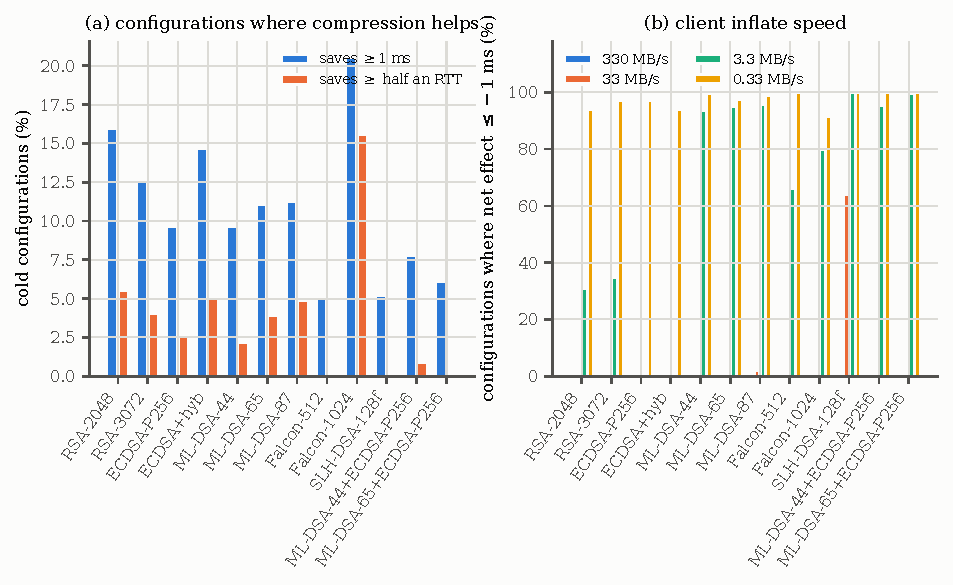
\includegraphics[width=\textwidth]{figures/fig_cc}
\caption{Certificate compression: (a) configurations where it helps; (b) configurations where it is net-harmful.}
\end{figure}

\clearpage
\section*{S3. Measurements (NVIDIA GX10: Cortex-X925 / Cortex-A725)}
\begin{table}[h]\centering\small
\caption{Per-operation CPU cost (ms): medians measured on a performance (Cortex-X925) and an efficiency (Cortex-A725) core.}
\resizebox{\textwidth}{!}{\begin{tabular}{@{}llrrrl@{}}
\toprule
Algorithm & Op. & X925 & A725 & A725/X925 & Implementation \\
\midrule
RSA-2048 & sign & 0.491 & 1.085 & 2.21 & OpenSSL 3.5.4 \\
RSA-2048 & verify & 0.0147 & 0.03163 & 2.15 & OpenSSL 3.5.4 \\
RSA-3072 & sign & 1.451 & 3.271 & 2.26 & OpenSSL 3.5.4 \\
RSA-3072 & verify & 0.0293 & 0.0648 & 2.21 & OpenSSL 3.5.4 \\
ECDSA-P256 & sign & 0.01446 & 0.02616 & 1.81 & OpenSSL 3.5.4 \\
ECDSA-P256 & verify & 0.04112 & 0.07835 & 1.91 & OpenSSL 3.5.4 \\
ML-DSA-44 & sign & 0.3594 & 0.753 & 2.10 & OpenSSL 3.5.4 \\
ML-DSA-44 & verify & 0.06804 & 0.1489 & 2.19 & OpenSSL 3.5.4 \\
ML-DSA-65 & sign & 0.586 & 1.225 & 2.09 & OpenSSL 3.5.4 \\
ML-DSA-65 & verify & 0.103 & 0.2289 & 2.22 & OpenSSL 3.5.4 \\
ML-DSA-87 & sign & 0.6691 & 1.438 & 2.15 & OpenSSL 3.5.4 \\
ML-DSA-87 & verify & 0.1589 & 0.3594 & 2.26 & OpenSSL 3.5.4 \\
Falcon-512 & sign & 0.1045 & 0.2057 & 1.97 & liboqs 0.14.0 \\
Falcon-512 & verify & 0.01755 & 0.0311 & 1.77 & liboqs 0.14.0 \\
Falcon-1024 & sign & 0.2114 & 0.4026 & 1.90 & liboqs 0.14.0 \\
Falcon-1024 & verify & 0.03098 & 0.05949 & 1.92 & liboqs 0.14.0 \\
SLH-DSA-128s & sign & 170.8 & 259.6 & 1.52 & OpenSSL 3.5.4 \\
SLH-DSA-128s & verify & 0.1614 & 0.2604 & 1.61 & OpenSSL 3.5.4 \\
SLH-DSA-128f & sign & 8.2 & 13.08 & 1.60 & OpenSSL 3.5.4 \\
SLH-DSA-128f & verify & 0.5058 & 0.7719 & 1.53 & OpenSSL 3.5.4 \\
\midrule
ECDHE-P256 & gen & 0.00845 & 0.01721 & 2.04 & OpenSSL 3.5.4 \\
ECDHE-P256 & derive & 0.03406 & 0.06565 & 1.93 & OpenSSL 3.5.4 \\
ECDHE-P256 & server & 0.04251 & 0.08286 & 1.95 & OpenSSL 3.5.4 \\
X25519 & gen & 0.01326 & 0.03127 & 2.36 & OpenSSL 3.5.4 \\
X25519 & derive & 0.0227 & 0.04522 & 1.99 & OpenSSL 3.5.4 \\
X25519 & server & 0.03596 & 0.07649 & 2.13 & OpenSSL 3.5.4 \\
X25519MLKEM768 & gen & 0.0311 & 0.07323 & 2.35 & OpenSSL 3.5.4 \\
X25519MLKEM768 & derive & 0.03734 & 0.08021 & 2.15 & OpenSSL 3.5.4 \\
X25519MLKEM768 & server & 0.04516 & 0.09852 & 2.18 & OpenSSL 3.5.4 \\
ML-KEM-768 & gen & 0.01784 & 0.04196 & 2.35 & OpenSSL 3.5.4 \\
ML-KEM-768 & derive & 0.01464 & 0.03499 & 2.39 & OpenSSL 3.5.4 \\
ML-KEM-768 & server & 0.0092 & 0.02203 & 2.40 & OpenSSL 3.5.4 \\
ML-KEM-1024 & gen & 0.02664 & 0.06338 & 2.38 & OpenSSL 3.5.4 \\
ML-KEM-1024 & derive & 0.01898 & 0.0458 & 2.41 & OpenSSL 3.5.4 \\
ML-KEM-1024 & server & 0.01183 & 0.02885 & 2.44 & OpenSSL 3.5.4 \\
\bottomrule
\end{tabular}
}
\end{table}

\begin{table}[h]\centering\small
\caption{DER sizes (bytes) of the generated certificates, their metadata, and the size predicted from the ECDSA-calibrated metadata.}
\resizebox{\textwidth}{!}{\begin{tabular}{@{}lrrrrrr@{}}
\toprule
Algorithm & Leaf DER & CA DER & Metadata (leaf/CA) & Predicted leaf & Predicted CA & Max error (\%) \\
\midrule
RSA-2048 & 1416 & 1227 & 862/673 & 1408 & 1217 & 0.81 \\
RSA-3072 & 1672 & 1483 & 862/673 & 1664 & 1473 & 0.67 \\
ECDSA-P256 & 1021 & 830 & 854/663 & 1021 & 830 & 0.00 \\
ML-DSA-44 & 4616 & 4427 & 858/669 & 4612 & 4421 & 0.14 \\
ML-DSA-65 & 6145 & 5956 & 858/669 & 6141 & 5950 & 0.10 \\
ML-DSA-87 & 8103 & 7914 & 858/669 & 8099 & 7908 & 0.08 \\
SLH-DSA-128s & 8768 & 8579 & 854/665 & 8768 & 8577 & 0.02 \\
SLH-DSA-128f & 18000 & 17811 & 854/665 & 18000 & 17809 & 0.01 \\
\bottomrule
\end{tabular}
}
\end{table}

\begin{table}[h]\centering\small
\caption{Compression ratio of real certificate chains: zlib level 9 vs.\ the model. The generated chains repeat names and extensions more than public chains, so classical chains compress better here than in the calibration set.}
\resizebox{\textwidth}{!}{\begin{tabular}{@{}lrrrrrrrr@{}}
\toprule
Algorithm & \multicolumn{2}{c}{$d=1$} & \multicolumn{2}{c}{$d=2$} & \multicolumn{2}{c}{$d=3$} & \multicolumn{2}{c}{$d=4$} \\
\cmidrule(lr){2-3} \cmidrule(lr){4-5} \cmidrule(lr){6-7} \cmidrule(lr){8-9}
 & zlib-9 & model & zlib-9 & model & zlib-9 & model & zlib-9 & model \\
\midrule
RSA-2048 & 0.76 & 0.81 & 0.67 & 0.77 & 0.61 & 0.75 & 0.58 & 0.75 \\
RSA-3072 & 0.80 & 0.83 & 0.73 & 0.81 & 0.68 & 0.80 & 0.65 & 0.79 \\
ECDSA-P256 & 0.64 & 0.73 & 0.53 & 0.67 & 0.44 & 0.65 & 0.40 & 0.64 \\
ML-DSA-44 & 0.93 & 0.94 & 0.91 & 0.93 & 0.89 & 0.93 & 0.88 & 0.93 \\
ML-DSA-65 & 0.95 & 0.95 & 0.93 & 0.95 & 0.92 & 0.95 & 0.92 & 0.95 \\
ML-DSA-87 & 0.96 & 0.97 & 0.95 & 0.96 & 0.94 & 0.96 & 0.94 & 0.96 \\
SLH-DSA-128s & 0.96 & 0.97 & 0.95 & 0.96 & 0.95 & 0.96 & 0.94 & 0.96 \\
SLH-DSA-128f & 0.98 & 0.98 & 0.98 & 0.98 & 0.98 & 0.98 & 0.97 & 0.98 \\
\bottomrule
\end{tabular}
}
\end{table}

\begin{table}[h]\centering\small
\caption{Real TLS 1.3 handshake flights (bytes, OpenSSL 3.5.4, mutual TLS) vs.\ the calibrated model with the same certificates, and loopback handshake time vs.\ modelled handshake CPU.}
\resizebox{\textwidth}{!}{\begin{tabular}{@{}lrrrrrrrr@{}}
\toprule
Suite (mutual TLS) & $d$ & CH & Server flight & Client flight & Model total & Error (\%) & Loopback (ms) & Model CPU (ms) \\
\midrule
RSA-2048 & 1 & 323 & 2075 & 1812 & 4202 & -0.19 & 2.00 & 1.13 \\
RSA-2048 & 4 & 323 & 5771 & 5508 & 11594 & -0.07 & 2.07 & 1.21 \\
RSA-3072 & 1 & 323 & 2459 & 2196 & 4970 & -0.16 & 4.21 & 3.10 \\
RSA-3072 & 4 & 323 & 6923 & 6660 & 13898 & -0.06 & 4.38 & 3.28 \\
ECDSA-P256 (baseline) & 1 & 290 & 1460 & 1231 & 2974 & -0.23 & 0.74 & 0.27 \\
ECDSA-P256 (baseline) & 4 & 290 & 3969 & 3737 & 7992 & -0.05 & 0.85 & 0.51 \\
ECDSA-P256 + hybrid KEM & 1 & 1466 & 2548 & 1231 & 5246 & 0.02 & 0.59 & 0.31 \\
ECDSA-P256 + hybrid KEM & 4 & 1466 & 5057 & 3737 & 10264 & 0.04 & 0.82 & 0.55 \\
ML-DSA-44 & 1 & 1434 & 8462 & 7176 & 17072 & 0.00 & 0.97 & 1.03 \\
ML-DSA-44 & 4 & 1434 & 21780 & 20494 & 43708 & 0.00 & 1.51 & 1.44 \\
ML-DSA-65 & 1 & 1434 & 10880 & 9594 & 21908 & 0.00 & 1.89 & 1.63 \\
ML-DSA-65 & 4 & 1434 & 28785 & 27499 & 57718 & 0.00 & 2.23 & 2.24 \\
ML-DSA-87 & 1 & 1818 & 14636 & 12870 & 29324 & 0.00 & 2.31 & 2.03 \\
ML-DSA-87 & 4 & 1818 & 38415 & 36649 & 76882 & 0.00 & 2.36 & 2.98 \\
\bottomrule
\end{tabular}
}
\end{table}

\clearpage
\section*{S4. Internet check, application objects and sensitivity}
\begin{table}[h]\centering\small
\caption{Real-Internet handshakes with X25519 and X25519MLKEM768 (100 interleaved rounds per server): median times, paired difference with bootstrap 95\,\% confidence interval, and extra bytes.}
\resizebox{\textwidth}{!}{\begin{tabular}{@{}lrrrrr@{}}
\toprule
Server & RTT (ms) & X25519 (ms) & X25519MLKEM768 (ms) & Paired difference (ms) & Extra bytes out/in \\
\midrule
cloudflare.com & 30 & 35.4 & 37.0 & 2.9 [1.2, 4.4] & 1176/1088 \\
www.google.com & 34 & 62.9 & 65.9 & 2.5 [0.1, 5.7] & 1176/1088 \\
\bottomrule
\end{tabular}
}
\end{table}

\begin{table}[h]\centering\small
\caption{Real signed application objects (bytes) against the model: JWS client assertion and access token, DPoP proof and XMLDSig over a pacs.008 document (signer certificate in \texttt{KeyInfo}).}
\resizebox{\textwidth}{!}{\begin{tabular}{@{}lrrrrrrrr@{}}
\toprule
Algorithm & \multicolumn{2}{c}{Client assertion} & \multicolumn{2}{c}{Access token} & \multicolumn{2}{c}{DPoP proof} & \multicolumn{2}{c}{XMLDSig} \\
\cmidrule(lr){2-3}\cmidrule(lr){4-5}\cmidrule(lr){6-7}\cmidrule(l){8-9}
 & real & model & real & model & real & model & real & model \\
\midrule
ECDSA-P256 & 381 & 536 & 549 & 796 & 518 & 732 & 2268 & 2270 \\
RSA-2048 & 637 & 782 & 805 & 1042 & 1104 & 1342 & 3055 & 3034 \\
ML-DSA-44 & 3527 & 3667 & 3695 & 3927 & 5883 & 6081 & 10182 & 10190 \\
ML-DSA-65 & 4712 & 4852 & 4880 & 5112 & 8206 & 8403 & 13406 & 13414 \\
ML-DSA-87 & 6470 & 6610 & 6638 & 6870 & 11101 & 11298 & 17774 & 17782 \\
SLH-DSA-128s & 10786 & 10915 & 10954 & 11175 & 10877 & 11053 & 22969 & 22978 \\
SLH-DSA-128f & 23095 & 23224 & 23263 & 23484 & 23186 & 23362 & 47585 & 47598 \\
\bottomrule
\end{tabular}
}
\end{table}

\begin{table}[h]\centering\small
\caption{Global sensitivity: largest first- and second-order variance-based indices of log latency and of the log post-quantum factor over the full factorial designs.}
\resizebox{\textwidth}{!}{\begin{tabular}{@{}lp{0.68\textwidth}@{}}
\toprule
Response & Largest first- and second-order indices \\
\midrule
log latency, wired & RTT (0.59), suite (0.28), suite x RTT (0.04), protocol (0.03), MTU (0.02) \\
log PQ factor, wired, all PQ suites & suite (0.68), RTT (0.12), suite x RTT (0.09), MTU (0.02), protocol (0.01) \\
log PQ factor, wired, ML-DSA and Falcon & RTT (0.20), MTU (0.18), suite (0.16), penalty (0.09), protocol (0.06) \\
log PQ factor, radio, all PQ suites & suite (0.67), protocol (0.07), suite x protocol (0.05), protocol x connection reuse (0.04), radio profile (0.03) \\
log PQ factor, radio, ML-DSA and Falcon & suite (0.23), protocol (0.15), SINR (0.14), radio profile (0.12), protocol x connection reuse (0.06) \\
\bottomrule
\end{tabular}
}
\end{table}

\begin{table}[h]\centering\small
\caption{Parameter uncertainty: SWIFT~MX, depth 2, 100\,Mbps, 30\,ms RTT, 4\,000 draws of certificate metadata, CPU scale (1--16$\times$), $\pi$, $\theta$ and initial window (\texttt{uncertainty.py}). Probabilities are shown in the median column.}
\begin{tabular}{@{}lrrr@{}}\toprule
Metric & Median & 5th pct & 95th pct \\\midrule
ML-DSA-65 latency (ms) & 179.6 & 115.1 & 238.5 \\
ML-DSA-65 factor over baseline & 1.46 & 1.19 & 1.72 \\
Falcon-512 factor & 1.05 & 1.01 & 1.23 \\
SLH-DSA-128f factor & 3.34 & 2.31 & 6.21 \\
SLH-DSA-128s factor & 25.6 & 8.2 & 79.4 \\
ML-DSA-65 cost per extra certificate (ms) & 20.5 & 3.5 & 27.9 \\
P(overhead $>$ crypto time) & 0.91 & \multicolumn{2}{c}{--} \\
P(Falcon $<$ ML-DSA $<$ SLH-f) & 1.00 & \multicolumn{2}{c}{--} \\
\bottomrule\end{tabular}

\end{table}

\begin{table}[h]\centering\small
\caption{Cost per operation of the primitives on the critical path (ms, median): Cortex-X925 (simulator default), Cortex-A725 and one core of an Intel Core i7-5600U (2.5\,GHz, AVX2, turbo off), same method and OpenSSL~3.5.4 (liboqs 0.14.0 for Falcon).}
\begin{tabular}{@{}llrrrr@{}}
\toprule
Primitive & Operation & X925 (ms) & A725 (ms) & x86 (ms) & x86/X925 \\
\midrule
RSA-2048 & sign & 0.491 & 1.09 & 0.835 & 1.7 \\
RSA-2048 & verify & 0.0147 & 0.0316 & 0.0334 & 2.3 \\
ECDSA-P256 & sign & 0.0145 & 0.0262 & 0.0402 & 2.8 \\
ECDSA-P256 & verify & 0.0411 & 0.0783 & 0.102 & 2.5 \\
ML-DSA-44 & sign & 0.359 & 0.753 & 1.05 & 2.9 \\
ML-DSA-44 & verify & 0.068 & 0.149 & 0.213 & 3.1 \\
ML-DSA-65 & sign & 0.586 & 1.22 & 1.72 & 2.9 \\
ML-DSA-65 & verify & 0.103 & 0.229 & 0.326 & 3.2 \\
ML-DSA-87 & sign & 0.669 & 1.44 & 1.95 & 2.9 \\
ML-DSA-87 & verify & 0.159 & 0.359 & 0.508 & 3.2 \\
Falcon-512 & sign & 0.105 & 0.206 & 0.361 & 3.4 \\
Falcon-512 & verify & 0.0176 & 0.0311 & 0.065 & 3.7 \\
SLH-DSA-128s & sign & 171 & 260 & 1.32e+03 & 7.7 \\
SLH-DSA-128s & verify & 0.161 & 0.26 & 1.3 & 8.1 \\
SLH-DSA-128f & sign & 8.2 & 13.1 & 63.1 & 7.7 \\
SLH-DSA-128f & verify & 0.506 & 0.772 & 3.79 & 7.5 \\
X25519 & key generation & 0.0133 & 0.0313 & 0.0513 & 3.9 \\
X25519 & derive & 0.0227 & 0.0452 & 0.0509 & 2.2 \\
ML-KEM-768 & key generation & 0.0178 & 0.042 & 0.0641 & 3.6 \\
ML-KEM-768 & encapsulate & 0.0092 & 0.022 & 0.04 & 4.3 \\
ML-KEM-768 & decapsulate & 0.0146 & 0.035 & 0.0608 & 4.2 \\
\bottomrule
\end{tabular}

\end{table}

\begin{table}[h]\centering\small
\caption{Error of the stack model against the testbed (model minus measured excess latency) by group of configurations: mean absolute error (MAE), root-mean-square error (RMSE), MAE as a percentage of the mean measured excess latency, and 95\% bootstrap interval of the MAE (2\,000 resamples of the configurations). The core grid is the set on which the two stack behaviours were identified (100\,Mbit/s, initial window 10); the rest was measured after the model was fixed. Reno, no loss, mutual TLS, direct path (\texttt{residual\_analysis.py}).}
\resizebox{\textwidth}{!}{\begin{tabular}{@{}llrrrrr@{}}
\toprule
Group & Value & $n$ & MAE (ms) & RMSE (ms) & MAE / mean excess (\%) & MAE 95\% interval (ms) \\
\midrule
 & all configurations & 226 & 1.65 & 2.16 & 1.2 & 1.48--1.83 \\
\midrule
 & core grid (100 Mbit/s, initial window 10) & 82 & 0.96 & 1.34 & 0.6 & 0.77--1.18 \\
 & away from the calibration point & 144 & 2.04 & 2.51 & 1.8 & 1.81--2.28 \\
\midrule
RTT (ms) & 5 & 24 & 0.95 & 1.31 & 4.9 & 0.63--1.33 \\
RTT (ms) & 30 & 178 & 1.84 & 2.34 & 1.6 & 1.63--2.05 \\
RTT (ms) & 100 & 24 & 0.92 & 1.30 & 0.2 & 0.57--1.31 \\
\midrule
MTU (B) & 1280 & 58 & 1.87 & 2.39 & 1.5 & 1.50--2.26 \\
MTU (B) & 1500 & 120 & 1.33 & 1.83 & 0.9 & 1.12--1.57 \\
MTU (B) & 9000 & 48 & 2.17 & 2.61 & 2.1 & 1.77--2.58 \\
\midrule
initial window & 10 & 154 & 1.32 & 1.80 & 0.9 & 1.13--1.52 \\
initial window & 32 & 72 & 2.35 & 2.79 & 2.2 & 2.01--2.70 \\
\midrule
chain depth & 1 & 60 & 1.72 & 2.21 & 1.4 & 1.36--2.06 \\
chain depth & 2 & 58 & 1.58 & 2.00 & 1.2 & 1.28--1.89 \\
chain depth & 3 & 54 & 1.59 & 2.17 & 1.1 & 1.21--1.98 \\
chain depth & 4 & 54 & 1.70 & 2.27 & 1.2 & 1.33--2.13 \\
\midrule
suite & ECDSA-P256 & 63 & 1.48 & 1.89 & 1.4 & 1.19--1.77 \\
suite & ECDSA + hybrid KEM & 15 & 0.64 & 0.64 & 0.5 & 0.60--0.67 \\
suite & ML-DSA-44 & 12 & 0.72 & 0.90 & 0.4 & 0.43--1.03 \\
suite & ML-DSA-65 & 62 & 1.89 & 2.38 & 1.4 & 1.54--2.25 \\
suite & ML-DSA-87 & 62 & 2.14 & 2.67 & 1.4 & 1.75--2.54 \\
suite & RSA-2048 & 12 & 0.95 & 1.38 & 0.7 & 0.40--1.51 \\
\bottomrule
\end{tabular}
}
\end{table}

\begin{figure}[h]\centering
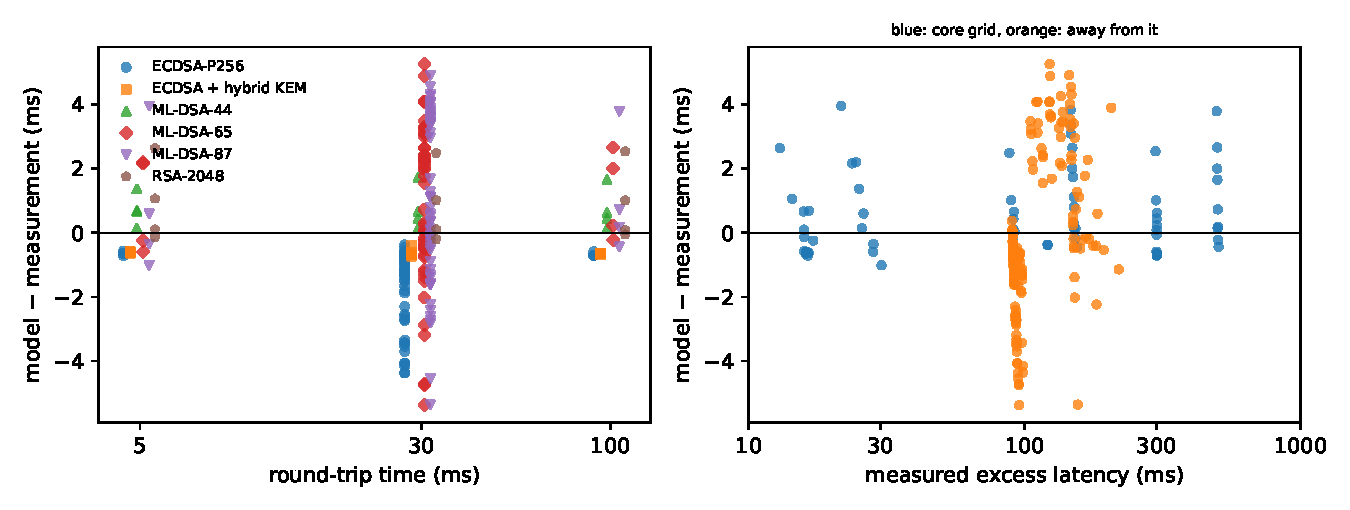
\includegraphics[width=\textwidth]{figures/fig_residuals}
\caption{Residuals of the stack model (model minus measurement) of the \resCoreN\ core-grid and \resAwayN\ off-grid testbed configurations against the round-trip time, by suite (left), and against the measured excess latency (right).}
\end{figure}

\begin{figure}[h]\centering
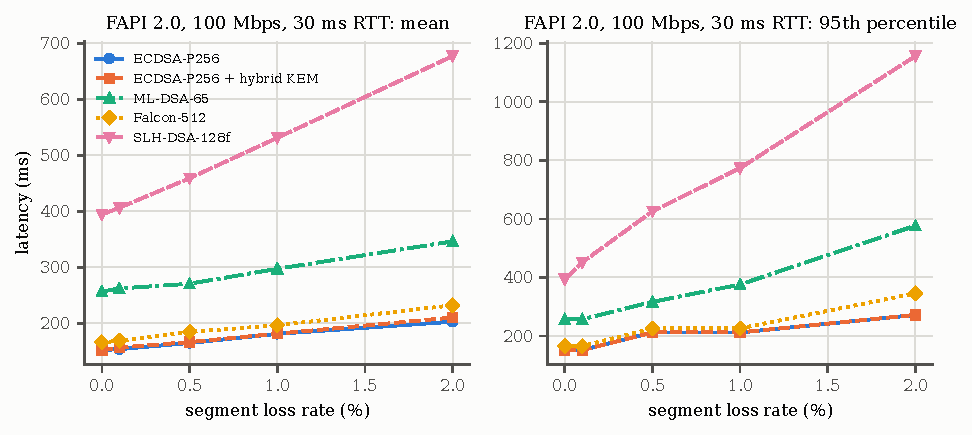
\includegraphics[width=\textwidth]{figures/fig_loss}
\caption{Wired-path packet loss: mean and 95th-percentile latency of a cold FAPI~2.0 transaction against the segment loss rate. Simulated with the idealised closed form (ideal segmentation, window $+n$ after every flight) and a 6\,ms penalty; not re-validated on the testbed.}
\end{figure}
\end{document}
